\documentclass[aspectratio=169]{beamer}
\usetheme{Madrid}
\usepackage{booktabs}
\usepackage{graphicx}
\usepackage{array}

\title{Branch Specialization Checkpoint}
\subtitle{Unlabeled Router Regularization}
\author{Branch Specialization Project}
\date{2026-05-22}

\begin{document}

\begin{frame}
  \titlepage
  \vspace{-0.5em}
  \begin{center}
    Checkpoint reason: generic gate regularizers did not reliably induce causal modularity.
  \end{center}
\end{frame}

\begin{frame}{Question}
  Previous checkpoint:
  \begin{itemize}
    \item weak role-label routing at weight 0.05 produced 5/5 causal modularity;
    \item gate compliance appeared before causal modularity.
  \end{itemize}

  \vspace{0.8em}
  This checkpoint asks:

  \begin{quote}
    Can unlabeled routing pressure produce similar branch-level functional
    modularity without local/induction role labels?
  \end{quote}
\end{frame}

\begin{frame}{Setup}
  Same local-vs-induction competition task:
  \begin{itemize}
    \item config: \texttt{learned\_token\_router};
    \item no scored-position role-label routing loss;
    \item five seeds per condition, 1200 training steps;
    \item branch modularity measured by branch ablation.
  \end{itemize}

  \vspace{0.6em}
  Unlabeled regularizers:
  \begin{itemize}
    \item entropy minimization: make per-position gates sharper;
    \item load balancing: keep global branch usage near 50/50;
    \item entropy plus load balancing.
  \end{itemize}
\end{frame}

\begin{frame}{Main Evidence}
  \begin{center}
  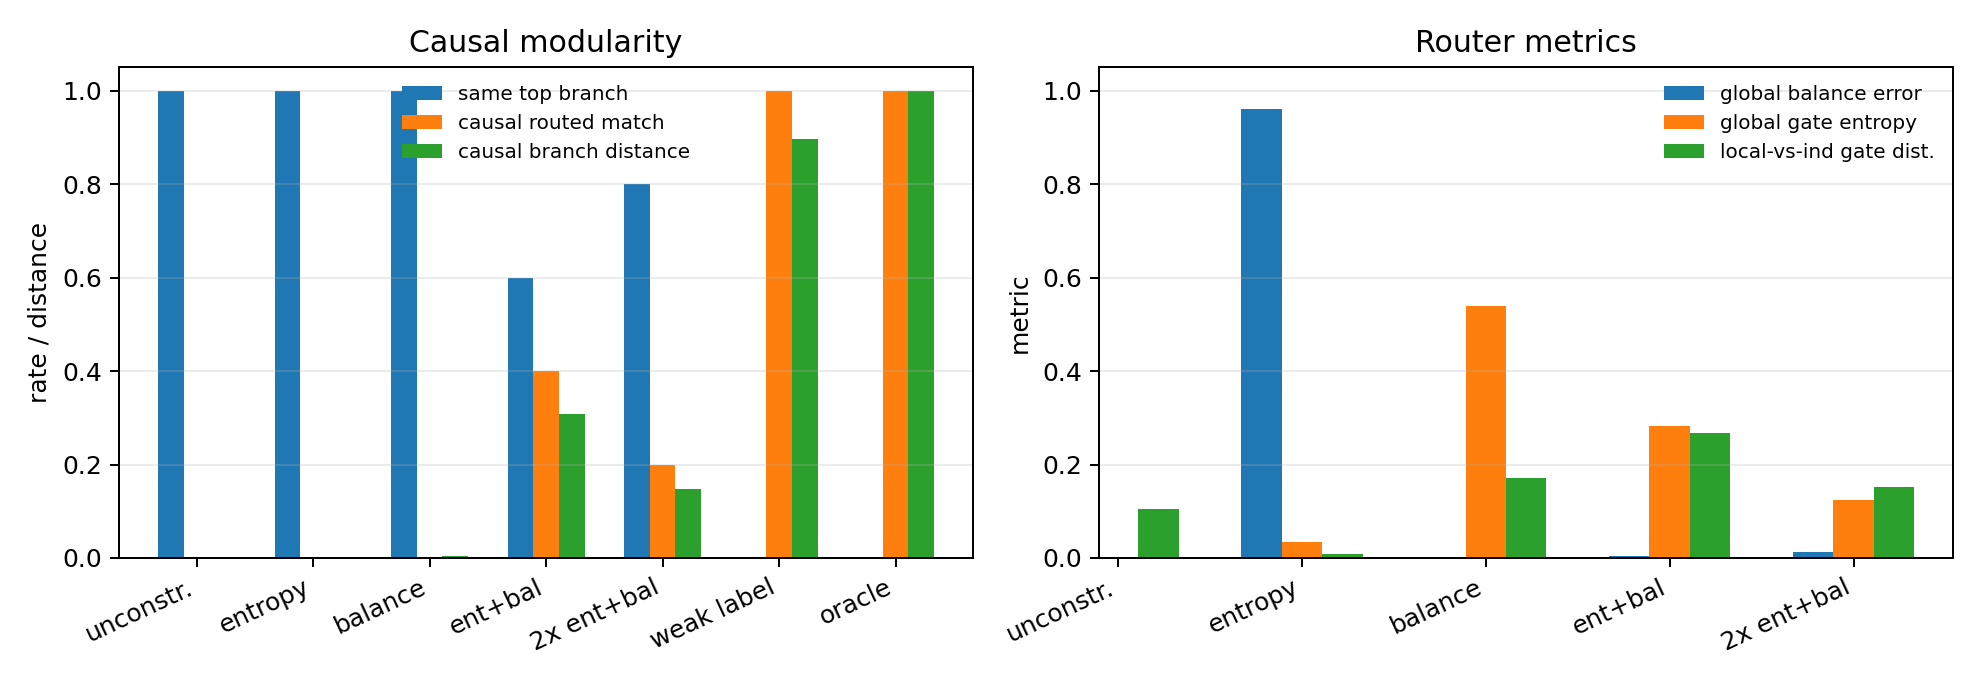
\includegraphics[width=0.92\linewidth]{figures/unlabeled_router_regularization.png}
  \end{center}

  \vspace{-0.4em}
  \small
  Entropy and balance regularizers change router statistics, but none approaches
  the weak-label or oracle causal modularity result.
\end{frame}

\begin{frame}{Causal Modularity}
  \begin{center}
  \scriptsize
  \begin{tabular}{lrrrrr}
    \toprule
    Condition & Local acc. & Ind. acc. & Same top & Routed match & Branch dist. \\
    \midrule
    \texttt{unconstrained} & 1.0000 & 0.9989 & 1.00 & 0.00 & 0.0006 \\
    \texttt{entropy} & 1.0000 & 0.9994 & 1.00 & 0.00 & 0.0002 \\
    \texttt{balance} & 1.0000 & 0.9993 & 1.00 & 0.00 & 0.0033 \\
    \texttt{ent+bal} & 1.0000 & 0.9993 & 0.60 & 0.40 & 0.3082 \\
    \texttt{2x ent+bal} & 1.0000 & 0.9984 & 0.80 & 0.20 & 0.1484 \\
    \texttt{weak label} & 0.9998 & 0.9983 & 0.00 & 1.00 & 0.8957 \\
    \texttt{oracle} & 1.0000 & 0.9988 & 0.00 & 1.00 & 1.0000 \\
    \bottomrule
  \end{tabular}
  \end{center}

  \vspace{0.5em}
  All unlabeled conditions solve the task, but remain far below weak labels on
  causal routed match.
\end{frame}

\begin{frame}{Router Metrics}
  \begin{center}
  \scriptsize
  \begin{tabular}{lrrrr}
    \toprule
    Condition & Balance error & Global entropy & Role gate dist. & Gate match \\
    \midrule
    \texttt{entropy} & 0.9597 & 0.0351 & 0.0095 & 0.00 \\
    \texttt{balance} & 0.0017 & 0.5385 & 0.1718 & 0.00 \\
    \texttt{ent+bal} & 0.0038 & 0.2830 & 0.2667 & 0.40 \\
    \texttt{2x ent+bal} & 0.0118 & 0.1247 & 0.1512 & 0.20 \\
    \bottomrule
  \end{tabular}
  \end{center}

  \vspace{0.7em}
  Load balancing can be almost perfect while local and induction remain
  functionally co-located.
\end{frame}

\begin{frame}{Failure Modes}
  \textbf{Entropy-only:}
  \begin{itemize}
    \item gates become sharp;
    \item each seed collapses both roles onto the same branch.
  \end{itemize}

  \vspace{0.5em}
  \textbf{Balance-only:}
  \begin{itemize}
    \item global branch usage is almost exactly 50/50;
    \item local and induction still depend on the same top branch in 5/5 seeds.
  \end{itemize}

  \vspace{0.5em}
  \textbf{Entropy plus balance:}
  \begin{itemize}
    \item sometimes finds a role split;
    \item remains mixed and far below weak labels.
  \end{itemize}
\end{frame}

\begin{frame}{Interpretation}
  \textbf{Supported in this toy setup:}
  \begin{itemize}
    \item Sharp routing is not functional modularity.
    \item Balanced routing is not functional modularity.
    \item Generic unlabeled gate regularizers are insufficient here.
  \end{itemize}

  \vspace{0.6em}
  \textbf{Current formulation:}
  \begin{quote}
    Structural branches and learned gates provide a substrate for modularity, but
    functional modularity needs role-informative routing pressure or equivalent
    task pressure.
  \end{quote}
\end{frame}

\begin{frame}{Decision}
  Stop sweeping generic gate regularizer weights on the current easy task.

  \vspace{0.8em}
  Next decisive experiment:
  \begin{quote}
    Increase role conflict or impose branch bottlenecks, then test whether
    unlabeled routing pressure begins to align with functional roles.
  \end{quote}

  \vspace{0.8em}
  The next result should distinguish whether the failure is due to the regularizer
  class or due to the task allowing cheap cohabitation.
\end{frame}

\begin{frame}{Sources and Provenance}
  \scriptsize
  \begin{itemize}
    \item Report: \texttt{doc/phase3\_toy\_unlabeled\_router\_regularization.md}
    \item Model script: \texttt{scripts/toy\_branch\_isolation\_intervention.py}
    \item Analysis script: \texttt{scripts/analyze\_unlabeled\_router\_regularization.py}
    \item Analysis output: \texttt{results/phase3\_toy\_unlabeled\_router\_regularization\_analysis/}
    \item Deck data snapshot: \texttt{presentations/2026-05-22-1551-unlabeled-router/data/}
  \end{itemize}
\end{frame}

\end{document}
